\section{Methods}\label{sec:methods}

The proposed prosthesis controller consists of two components. The first is an
Extended Kalman Filter (EKF) that estimates the gait phase, defined as the
percent of stance completed so far (\cref{sec:gpekf}). Ideally, the phase
estimate starts at zero at heel strike and reaches one precisely at toe-off. The
second component is a set of control surfaces, which are functions of phase and
phase velocity, that provide desired knee and ankle angles, velocities, and feed
forward torques for generating the prosthesis stance behavior
(\cref{sec:ctrl_surfs}).

\subsection{GP-EKF for estimating phase}\label{sec:gpekf}

In contrast to the previously described phase variable approach for phase
estimation in prostheses~\citep{quintero2016preliminary}, which uses a single
source of information, we take a sensor-fusion approach and combine angle and
velocity information from the hip, knee, and ankle joints of the prosthetic
limb.  An IMU mounted to the thigh portion of CMU's powered knee-and-ankle
prosthesis provides information about the user's hip motion, and encoders on the
prosthesis provide information about the knee and ankle joints. We use these
observations in an Extended Kalman filter (EKF) to estimate the phase and phase
velocity during stance. The EKF assumes the linear, discrete time phase dynamics
\begin{align}
    x_t = \begin{bmatrix} \phi_t \\ \dot{\phi}_t \end{bmatrix} 
        &= \begin{bmatrix} 1 & \Delta t \\ 0 & 1 \end{bmatrix} 
            \begin{bmatrix} \phi_{t-1} \\ \dot{\phi}_{t-1} \end{bmatrix} + w_t
            \label{eq:dyn_mdl} \\
        &= A x_{t-1}, \notag
\end{align}
where $\phi$ is the phase, $\dot{\phi}$ is the rate of change of phase, $\Delta
t$ is the integration time step and $w_t \sim \mathcal{N}(0, Q)$. We set
\begin{align}
    Q = \begin{bmatrix} 0 & 0 \\ 0 & \sigma_{\dot{\phi}}^2 \end{bmatrix},
\end{align}
with $\sigma_{\dot{\phi}}^2 = 1\tn{e}{-7}$. These dynamics encode the
assumption that phase should evolve continuously, at a roughly constant rate.

Observations of the prosthesis-side hip, knee, and ankle angles and velocities
inform the evolution of the above dynamics. For the joint angles, the
observation models are of the form
\begin{align}
    z_t^{\theta_j} = h^{\theta_j}(x_t) + v_t^{\theta_j}
        = \mathrm{GP}_\mu^{\theta_j}\left(\phi_t \right) + v_t^{\theta_j},
\end{align}
where $\mathrm{GP}_\mu^{\theta_j}$ is the mean of a learned Gaussian Process
(GP) model of the angle of joint $j$ as a function of the phase $\phi$ and
$v_t^{\theta_j} \sim \mathcal{N} \left(0,
\mathrm{GP}_{\sigma^2}^{\theta_j}(\phi_t) \right)$. Here,
$\mathrm{GP}_{\sigma^2}^{\theta_j}$ is the variance of the same learned GP
model.

Similarly, for the joint velocities we use an observation model of the form
\begin{align}
    \begin{split}
        z_t^{\nicefrac{d \theta_j}{d \phi}}
            &= h^{\nicefrac{d \theta_j}{d \phi}}(x_t) 
                + v_t^{\nicefrac{d \theta_j}{d \phi}} \dot{\phi}_t \\
            &= \left( \mathrm{GP}_\mu^{\nicefrac{d \theta_j}{d \phi}} 
            \left(\phi_t \right) + v_t^{\nicefrac{d \theta_j}{d \phi}} \right) 
            \dot{\phi}_t
    \end{split}
\end{align}
where $\mathrm{GP}_\mu^{\nicefrac{d \theta_j}{d \phi}}$ is the mean of a
Gaussian Process model of the velocity of joint $j$ (in units of $\nicefrac{d
\theta_j}{d \phi}$) as a function of $\phi$. In addition, $v_t^{\nicefrac{d
\theta_j}{d \phi}} \sim \mathcal{N} \left(0, \mathrm{GP}_{\sigma^2}^{\nicefrac{d
\theta_j}{d \phi}}(\phi_t) \right)$, where $\mathrm{GP}_{\sigma^2}^{\nicefrac{d
\theta_j}{d \phi}}$ is the variance of the same learned GP model for joint
velocity.

To train the GP observation models, the algorithm maintains a training data set
of stance gait data. The training data set includes the joint angles and
velocities (in units of $\nicefrac{d \theta_j}{d\phi}$) sampled at
\unit[100]{Hz} as well as the actual corresponding phases and phase velocities
during stance. We assume that, in hindsight, the actual phase increased linearly
from zero at heel strike to one at toe off and that the actual phase velocity
was constant during stance and equal to $1/T_n$, where $T_n$ is the duration of
the completed stance phase. We retrain the GP models using this gait data after
every five completed steps. To ensure that the test-time performance of the
Gaussian Process models does not degrade as more training data accumulates, we
employ the fully independent training conditional (FITC) approximation of the
GP~\citep{snelson2007local}. This approximation represents the GP using a
fixed-size active set of training points. (We use 25 points in our
approximation).

With the learned GP observation models, we follow the GP-EKF procedure proposed
by~\citet{ko2009gp} to obtain an estimate of phase and phase velocity. In this
procedure, we first \emph{predict} the next state distribution by propagating
the mean $\hat{x}_{t-1|t-1}$ and covariance $\Sigma_{t-1|t-1}$ of the state
using the dynamics model provided by \cref{eq:dyn_mdl},
\begin{align}
    \hat{x}_{t|t-1} &= A \hat{x}_{t-1|t-1} \label{eq:ekf_predict_mean}\\
    \Sigma_{t|t-1} &= A \Sigma_{t-1|t-1} A^T + Q. \label{eq:ekf_predict_cov}
\end{align}

Next, we \emph{update} the state distribution estimate given measurements $z_t$
of the joint angles and velocities using the following equations and the GP
observation models $h_t(x_t)$.
\begin{align}
    K_t &= \Sigma_{t|t-1} H_t^T {\left( H_t \Sigma_{t|t-1} H_t^T 
        + M_t R M_t^T \right)}^{-1} \\
    \hat{x}_{t|t} &= \hat{x}_{t|t-1} + K_t \left( z_t 
        - h \left(\hat{x}_{t|t-1} \right) \right) \\
    \Sigma_{t|t} &= \left(I - K_t H_t \right) \Sigma_{t|t-1}
\end{align}
where,
\begin{align}
    h(x_t) &= \begin{bmatrix} 
        \mathrm{GP}_\mu^{\theta_h}(\phi_t) \\
        \mathrm{GP}_\mu^{\theta_k}(\phi_t) \\
        \mathrm{GP}_\mu^{\theta_a}(\phi_t) \\
        \mathrm{GP}_\mu^{\nicefrac{d \theta_h}{d \phi}}(\phi_t) \dot{\phi}_t  \\
        \mathrm{GP}_\mu^{\nicefrac{d \theta_k}{d \phi}}(\phi_t) \dot{\phi}_t  \\
        \mathrm{GP}_\mu^{\nicefrac{d \theta_a}{d \phi}}(\phi_t) \dot{\phi}_t
        \end{bmatrix}
\end{align}
\begin{align}
    H_t &= \left. \frac{\partial h}{\partial x} \right|_{\hat{x}_{t|t-1}}
        = \begin{bmatrix} 
        \left. \nicefrac{\partial \mathrm{GP}_\mu^{\theta_h}}{\partial \phi_t}
            \right|_{\phi_t} & 0 \\
        \left. \nicefrac{\partial \mathrm{GP}_\mu^{\theta_k}}{\partial \phi_t}
            \right|_{\phi_t} & 0 \\
        \left. \nicefrac{\partial \mathrm{GP}_\mu^{\theta_a}}{\partial \phi_t}
            \right|_{\phi_t} & 0 \\
        \left. \nicefrac{\partial 
            \mathrm{GP}_\mu^{\nicefrac{d \theta_h}{d \phi}}}
            {\partial \phi_t} \right|_{\phi_t} \dot{\phi}_t & 
            \mathrm{GP}_\mu^{\nicefrac{d \theta_h}{d \phi}} \\
        \left. \nicefrac{\partial 
            \mathrm{GP}_\mu^{\nicefrac{d \theta_k}{d \phi}}}
            {\partial \phi_t} \right|_{\phi_t} \dot{\phi}_t & 
            \mathrm{GP}_\mu^{\nicefrac{d \theta_k}{d \phi}} \\
        \left. \nicefrac{\partial 
            \mathrm{GP}_\mu^{\nicefrac{d \theta_a}{d \phi}}}
            {\partial \phi_t} \right|_{\phi_t} \dot{\phi}_t & 
            \mathrm{GP}_\mu^{\nicefrac{d \theta_a}{d \phi}}
        \end{bmatrix} \label{eq:H_ekf}
\end{align}
\begin{align}
    M_t &= \left. \frac{\partial h}{\partial v_t} \right|_{\hat{x}_{t|t-1}} 
        = \begin{bmatrix}
        I_{3 \times 3} & 0 \\ 0 & \dot{\phi}_t I_{3 \times 3}
        \end{bmatrix}
\end{align}
\begin{align}
    \begin{split}
    R_t &= \tn{blkdiag} \left(\mathrm{GP}_{\sigma^2}^{\theta_h}(\phi_t),
        \mathrm{GP}_{\sigma^2}^{\theta_k}(\phi_t), 
        \mathrm{GP}_{\sigma^2}^{\theta_a}(\phi_t), \right. \\
        & \qquad \left. \mathrm{GP}_{\sigma^2}^{\nicefrac{d \theta_h}{d\phi}}
            (\phi_t),
        \mathrm{GP}_{\sigma^2}^{\nicefrac{d \theta_k}{d\phi}}(\phi_t),
        \mathrm{GP}_{\sigma^2}^{\nicefrac{d \theta_a}{d\phi}}(\phi_t) \right)
    \end{split}
\end{align}
Due to the linearity of Gaussian processes and differentiation, we can
analytically obtain derivatives required by \cref{eq:H_ekf} using the methods
provided by \citet{solak2003derivative}. 

\begin{figure*}[t]
    \centering
    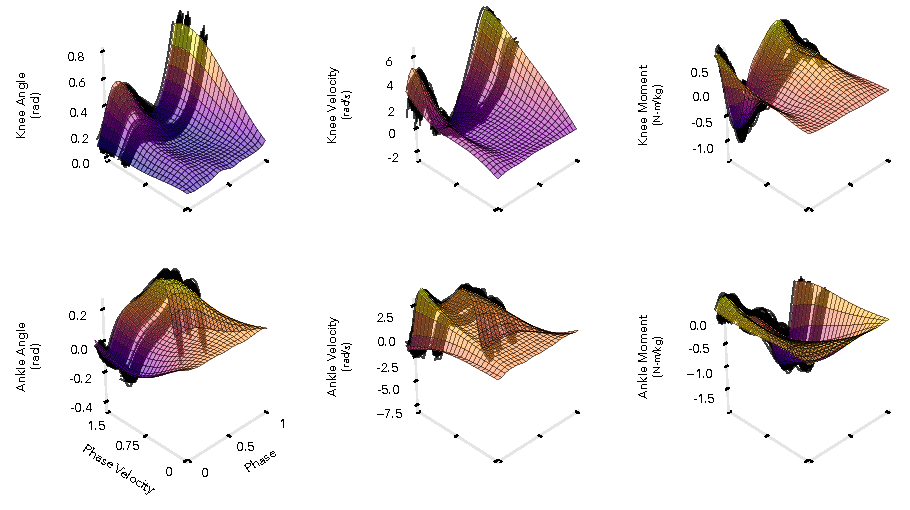
\includegraphics[width=\textwidth]{control_surfaces}
    \caption{Examples of learned control surfaces. We fit the surfaces to gait
    data from \citet{moore2015elaborate}. This data includes information for
    three speeds, \unitfrac[0.8, 1.2, and 1.6]{m}{s}, which are shown as the
    clustered trajectories in the above panels.  For an automatic transition to
    standing, the surfaces are additionally fit to virtual data that causes the
    joint angles to approach \unit[5]{deg}, the velocities to approach
    \unitfrac[0]{deg}{s}, and the joint torques to approach \unit[0]{N-m} as the
    phase velocity goes to zero.}\label{fig:control_surf}
\end{figure*}

Finally, we reset the state distribution at heel strike to
\begin{align}
    \hat{x}_0 = \begin{bmatrix} 0 \\ 1/T_{n-1} \end{bmatrix}, \quad \Sigma_0 
        =  0_{2 \times 2}, \label{eq:init_cond_ekf}
\end{align}
where $T_{n-1}$ is the duration of the previous stance.

\subsection{Control Surfaces}\label{sec:ctrl_surfs}

We use the mean estimates of the phase $\phi$ and phase velocity $\dot{\phi}$ as
the inputs into learned control surfaces that provide the desired knee and ankle
angles, velocities, and feed-forward torques (Fig.~\ref{fig:control_surf}). The
final desired torques applied to the prosthesis are then given by 
\begin{align}
    \tau_d = k_\tn{p} \left(\theta_\tn{d}(\phi, \dot{\phi}) - \theta \right) 
        + k_\tn{d} \left(\dot{\theta}_\tn{d}(\phi, \dot{\phi}) 
            - \dot{\theta} \right)
        + \tau_\tn{ff}(\phi, \dot{\phi}), \label{eq:pdandff}
\end{align}
where $\theta_\tn{d}$, $\dot{\theta}_\tn{d}$, and $\tau_\tn{ff}$ are the
learned control surfaces as functions of the estimated phase and phase velocity,
$k_\tn{p}$ and $k_\tn{d}$ are proportional and derivative gains,
and $\theta$ and $\dot{\theta}$ are the actual joint angle and velocity.

We learned the control surfaces $\theta_\tn{d}, \dot{\theta}_\tn{d}$ and
$\tau_\tn{ff}$, by regressing the gait data provided
by~\citet{moore2015elaborate} for several subjects walking at three speeds,
\unitfrac[0.8, 1.2, and 1.6]{m}{s}. We were able to learn the control surfaces
using the data from nine subjects. For each subject, we split the gait data into
individual stance phases and extracted the knee and ankle angles, velocities,
and joint torques.  We also assumed that during each stance, the actual phase
increased linearly from zero at heel strike to one at toe off and the phase
velocity during stance was constant and equal to $1/T$, where $T$ is the
duration of stance. We again used sparse GP regression with the FITC
approximation to regress the knee and ankle angles, velocities, and torques
versus the phase and phase velocity. In this case, we used 100 active vectors to
approximate each GP.\ 

The gait data spans the whole range of phases $([0, 1])$ but not the whole range
of physiological phase velocities, as the gait speed only varies between
\unitfrac[0.8 and 1.6]{m}{s}. To ensure the control surfaces generate smooth
behaviors at slower speeds and when standing still $(\dot{\phi} = 0)$, we
additionally trained the GPs on a grid spanning $\phi \in [0, 1]$ and
$\dot{\phi} \in [0, \min(\dot{\phi}_\textrm{data set})]$ with \emph{virtual}
training values derived from interpolating between the average trajectory at
\unitfrac[0.8]{m}{s} and desired values at $\dot{\phi} = 0$. When $\dot{\phi} =
0$, the desired joint angles, velocities and torques were set to \unit[5]{deg},
\unitfrac[0]{deg}{s}, and \unit[0]{N-m},  respectively, thereby creating a
smooth transition to a standing mode. \Cref{fig:control_surf} shows examples of
the resulting control surfaces derived from one subject's data.

\subsection{Experimental Protocol}\label{sec:exp}

\begin{marginfigure}
    \centering
    \includegraphics[width=\columnwidth]{prosthesis}
    \caption{CMU powered prosthesis used in experiments. The prosthesis
    has brushless motors at the knee and ankle joints, series elastic actuators
    for torque control, and an IMU mounted to the thigh portion to measure
    residual limb angle.}\label{fig:prosthesis}
\end{marginfigure}

We evaluated the naturalness of gait and the robustness of our proposed
controller in experiments conducted with seven able-bodied subjects, and an
amputee subject. We additionally present data from an experienced user of the
prosthesis (first author of paper), whose gait characteristics induced a
different response from the prosthesis. All subjects provided informed consent
to IRB-approved protocols.  The amputee subject wore the powered prosthesis
prototype shown in~\cref{fig:prosthesis}, while able-bodied subjects used a
shortened version of the prosthesis attached via an L-shaped adapter. (for more
information on prosthesis specifications see~\citep{thatte2018method}). All
subjects had at least six hours of prior practice walking on the prosthesis. The
able-bodied subjects walked without assistance from handrails, while the amputee
subject used the handrails for balance.

We compared our proposed control method to a stance control based on a
neuromuscular model of human neurophysiology~\citep{thatte2018method} and to
finite state impedance control~\citep{lawson2014robotic}. For these controllers,
we generated parameter sets by fitting control parameters to the same nine
subjects' gait data used to generate the control surfaces described in
\cref{sec:ctrl_surfs}. For neuromuscular control, we used the black-box CMA-ES
optimizer~\citep{hansen2006cma} to fit the control parameters as described
in~\citep{thatte2018method}. For impedance control, we used robust RANSAC linear
regression~\citep{fischler1981random} to fit the stiffness, damping, and angle
offset parameters within the three discrete phases of stance. The transition
between phases 1 and 2 was based on the knee angle crossing a threshold, while
the transition between phases 2 and 3 was based on the ankle angle crossing a
threshold. We set these thresholds so that 95\% of steps in the gait data
transition through all three phases. Prior to beginning the experiments,
subjects walked with each of the nine control surfaces (parameter sets) for each
controller and indicated their preferred settings. All three stance control
strategies were paired with the same swing control strategy, in which minimum
jerk trajectories for the knee and ankle are generated at toe-off and tracked
with PD-feedback combined with a model-based feed forward term as
in~\citep{lenzi2014speed}. In total, we conducted four experiments: 

(1) A test of the ability of each control strategy to reproduce a normal walking
gait pattern.  Able-bodied subjects walked without the use of handrails
\unitfrac[0.8]{m}{s} and the amputee subject used the handrails and walked at
\unitfrac[0.6]{m}{s}.  All subjects walked with their preferred parameters for
each controller for one minute. We compared the resulting prosthesis knee and
ankle kinematics and kinetics to able-bodied gait data~\citep{bovi2011multiple}
to determine the naturalness of gait.

(2) A comparison of the robustness of the three controllers to ground height
disturbances. We simulated a ground disturbance by having subjects step on
\unit[3]{cm} blocks placed on the treadmill. We tested the controllers in a
random order in an ABCCBA sequence.  In each trial, the subjects stepped on
blocks 20 times. We recorded the number of falls, defined as instances when
subject needed support from either the handrails or a ceiling mounted harness to
regain balance.

\begin{comment}
Additionally, subjects frequently experienced a problem where the prosthesis
knee collapsed towards the end of stance when the blocks were near the heel.
Therefore, we also looked at the number of times the knee flexion angle at toe
off was abnormally large when stepping on a block. Here we defined an abnormal
flexion angle as being greater than three median absolute deviations away from
the median toe off knee angle during undisturbed walking.
\end{comment}

(3) A test of the adaptability of the phase estimate.  To test the adaptability,
we had subjects use the proposed GP-EKF control while the treadmill speed varied
sinusoidally between \unitfrac[0.4 and 1.2]{m}{s} with a \unit[20]{s} period. We
compared the phase and phase velocity estimates given by the EKF filter to the
true phase, assumed to increase linearly from zero at heel strike to one at toe
off, and the true phase velocity, assumed to equal $1/T_n$, where $T_n$ is the
duration of the current stance. As a baseline, we compared the EKF to time-based
phase and phase velocity estimates, which assume the duration of the current
stance will be the same as the previous stance, resulting in the phase and phase
velocity estimates
\begin{align}
    \phi_\textrm{time based} &= t_n/T_{n-1} \\
    \dot{\phi}_\textrm{time based} &= 1/T_{n-1}, \label{eq:init_cond_time}
\end{align}
where $t_n$ is the time after heel-strike of the current stance and $T_{n-1}$ is
the duration of the last stance. 

(4) Finally, a test of the ability of the GP-EKF control to respond to sudden
treadmill stops. If the subject stops his or her gait, then the phase estimate
should stabilize and the phase velocity should trend towards zero. The
corresponding desired joint angles should approach \unit[5]{deg} as shown in
\cref{fig:control_surf}. 

We assess significant differences between conditions via the two-sided paired
Wilcoxon signed rank test~\citep{gibbons2011nonparametric}. Experienced subject
data was not considered for significance testing.
